\documentclass[12pt,a4paper]{article}

% ---- Engine: compile with XeLaTeX (uses OpenType system fonts) ----
\usepackage[margin=2.35cm,headsep=14pt]{geometry}
\usepackage{graphicx}
\usepackage[table]{xcolor}
\usepackage{booktabs}
\usepackage{longtable}
\usepackage{array}
\usepackage{colortbl}
\usepackage{amsmath,amssymb}
\usepackage{enumitem}
\usepackage{setspace}
\usepackage{textcomp}
\usepackage{fontspec}
\usepackage{microtype}
\usepackage{fancyhdr}
\usepackage{titlesec}
\usepackage{caption}
\usepackage{parskip}
\usepackage[hidelinks,colorlinks=true,linkcolor=acc,urlcolor=acc,citecolor=acc]{hyperref}

% ---- Modern, pleasant fonts (TeX Gyre + DejaVu) ----
\setmainfont{TeX Gyre Pagella}                      % elegant Palatino-style body
\setsansfont{TeX Gyre Heros}[Scale=0.94]           % clean Helvetica-style headings
\setmonofont{DejaVu Sans Mono}[Scale=0.86]         % code / keys

% ---- Refined palette ----
\definecolor{acc}{HTML}{0F766E}     % deep teal accent
\definecolor{acc2}{HTML}{B45309}    % warm amber secondary
\definecolor{ink}{HTML}{1F2933}     % soft near-black body text
\definecolor{ink2}{HTML}{475569}    % muted slate
\definecolor{rule}{HTML}{D7DEDC}    % hairline rule grey
\definecolor{band}{HTML}{F1F6F5}    % subtle table band
\definecolor{codebg}{HTML}{F2F5F5}
\AtBeginDocument{\color{ink}}

\chardef\rawus=`\_
\DeclareRobustCommand{\code}[1]{{\ttfamily\small\def\_{\rawus\allowbreak}#1}}
\DeclareRobustCommand{\file}[1]{{\ttfamily\small\def\_{\rawus\allowbreak}#1}}
\DeclareRobustCommand{\key}[1]{{\ttfamily\small\color{acc2}\def\_{\rawus\allowbreak}#1}}
\newcommand{\nm}{\,nm}
\newcommand{\um}{\ensuremath{\mu\mathrm{s}}}
\setlength{\emergencystretch}{3em}

\setlist{itemsep=2pt,topsep=3pt}

% ---- Headings: sans, accented, with a hairline rule under sections ----
\titleformat{\section}[hang]
  {\sffamily\LARGE\bfseries\color{acc}}{\thesection}{0.6em}{}
  [\vspace{2pt}{\color{rule}\titlerule[1pt]}]
\titleformat{\subsection}
  {\sffamily\large\bfseries\color{ink}}{\thesubsection}{0.55em}{}
\titleformat{\paragraph}[runin]
  {\sffamily\bfseries\color{acc2}}{}{0pt}{}
\titlespacing*{\section}{0pt}{18pt}{8pt}
\titlespacing*{\subsection}{0pt}{12pt}{4pt}

% ---- Captions: small sans, accented label ----
\captionsetup{font=small,labelfont={sf,bf,color=acc},textfont={color=ink2},skip=6pt}

% ---- Tables: airier rows, soft hairlines ----
\setstretch{1.3}                 % body line spacing (between 1.25 and 1.5)
\renewcommand{\arraystretch}{1.12}
\arrayrulecolor{rule}
\setlength{\arrayrulewidth}{0.5pt}

% ---- Running head / foot ----
\pagestyle{fancy}\fancyhf{}
\lhead{\sffamily\small\color{ink2}Multi-Device Spectrum Analyzer}
\rhead{\sffamily\small\color{ink2}User \& Reference Manual}
\cfoot{\sffamily\small\color{ink2}\thepage}
\renewcommand{\headrulewidth}{0.5pt}
\renewcommand{\footrulewidth}{0pt}
\renewcommand{\headrule}{\hbox to\headwidth{\color{rule}\leaders\hrule height \headrulewidth\hfill}}

\newcommand{\fig}[3]{%
  \begin{figure}[ht]\centering
  \includegraphics[width=#2\linewidth]{figs/#1}
  \caption{#3}\label{fig:#1}\end{figure}}

\begin{document}

\begin{titlepage}
\sffamily
\thispagestyle{empty}
\noindent{\color{acc}\rule{\linewidth}{3pt}}\par
\vspace{1.6cm}
\noindent{\color{ink2}\large Technical \& User Reference Manual}\par
\vspace{0.5cm}
\noindent{\bfseries\color{acc}\fontsize{34}{38}\selectfont Multi-Device\\[2pt] Spectrum Analyzer}\par
\vspace{0.5cm}
\noindent{\color{ink}\Large PASCO PS-2600A\, \textbullet\, Ocean HDX\, \textbullet\, ASEQ LR-2T\, \textbullet\, Demo}\par
\vspace{0.4cm}
\noindent{\color{rule}\rule{\linewidth}{1pt}}\par
\vspace{1.2cm}
\begin{center}
\setlength{\fboxsep}{6pt}%
{\color{rule}\fbox{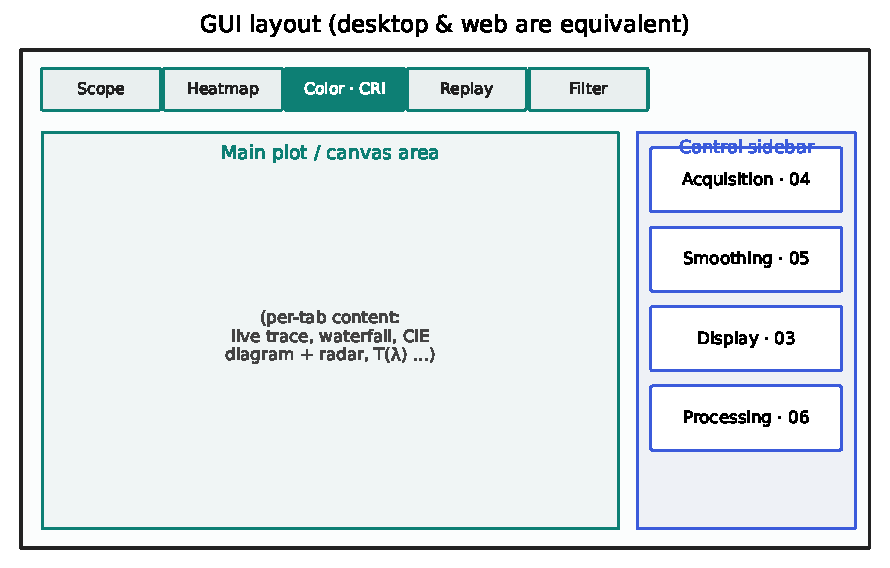
\includegraphics[width=0.9\linewidth]{figs/fig_gui_overview.pdf}}}
\end{center}
\vfill
\noindent\begin{minipage}{\linewidth}\color{ink2}\normalsize\rmfamily
A PyQt6 desktop application and FastAPI\,/\,WebSocket web client for live
spectroscopy, colorimetry (CIE\,/\,CRI\,/\,TM-30\,/\,CQS) and optical-filter
characterization across four spectrometer back-ends that share a single,
device-agnostic science core.
\end{minipage}\par
\vspace{0.9cm}
\noindent{\color{acc}\rule{\linewidth}{3pt}}\par
\vspace{4pt}
\noindent{\color{ink2}\small Generated \today\quad\textbullet\quad English}
\end{titlepage}

\tableofcontents
\clearpage

% =====================================================================
\section{Overview}
This program turns four different spectrometers into one consistent
instrument. The same window (and the same numbers) work whether you have a
PASCO PS-2600A CCD on USB, an Ocean Optics HDX, an ASEQ/Lasertack LR-2T, or no
hardware at all (the built-in \emph{Demo (virtual)} device). Every USB protocol
was reverse-engineered from scratch; there are no vendor SDKs in the loop.

\medskip
There are two front-ends that share one science core:
\begin{itemize}
  \item \textbf{Desktop} --- \file{PS-2600A\_Pro.py}, a PyQt6 + pyqtgraph GUI.
  \item \textbf{Web} --- \file{web\_server.py}, a FastAPI + WebSocket server with a
        browser client (\file{index.html} / \file{app.js} / \file{styles.css}, a
        uPlot scope and canvas-drawn heatmap\slash CIE\slash radar).
\end{itemize}
Because both call the identical engines (\file{color\_science.py},
\file{filter\_analysis.py}), a report exported from the web and one exported from
the desktop contain the same values.

\medskip
\textbf{What it does:} live scope with overlays (CSV background reference,
freeze-to-grey, difference-vs-freeze, peak-hold envelope, persistence/afterglow);
a time-lapse heatmap (waterfall); CIE~1931 colorimetry
(CCT, Duv, $x,y$, $u',v'$, CRI~Ra + R1--R15); IES TM-30-18 (Rf, Rg, 16 hue bins,
colour-vector graphic, 99-sample fidelity) and CQS (Qa/Qf/Qg); optical-filter
characterization (transmission, type, peak/centre $\lambda$, FWHM, 50\,\% edges,
10--90\,\% edge steepness, blocking, optical density); PDF/PNG/CSV report export; a
25-spectrum reference library; dark-current correction; spectral-response
compensation; auto-exposure; a simple fast-preview mode; optional temporal and
spatial smoothing; and (web) a CSV waterfall replay player.

\subsection{How to run}
\begin{quote}\ttfamily\small
python PS-2600A\_Pro.py\hfill\# desktop GUI (entry point)\\
python web\_server.py\hfill\# headless web server (FastAPI + WebSocket)\\
set FP\_DEBUG=1 \&\& python web\_server.py\hfill\# Windows: per-frame fast-preview log
\end{quote}

\textbf{Dependencies} (\file{requirements.txt}): PyQt6, pyqtgraph, numpy, scipy.
Optional but recommended:
\begin{itemize}
  \item \textbf{matplotlib} --- CIE diagram fill and the PDF/PNG report renderers.
        Without it, CSV export still works; PDF/PNG return a hint.
  \item \textbf{colour-science} (\code{pip install colour-science}) --- enables the
        IES TM-30-18 and CQS sub-tab and \code{/api/tm30}. Everything else
        (CRI, CIE, reports minus TM-30) is unaffected if it is missing.
  \item \textbf{pyusb + libusb-package} --- Ocean HDX. \textbf{hid} --- LR-2T.
        PASCO needs WinUSB (via Zadig) on Windows.
\end{itemize}
The Demo device needs only numpy, so the application is always usable for
learning and testing with no hardware attached.

% =====================================================================
\section{System architecture}
\fig{fig_architecture.pdf}{0.92}{Module layout and the frame data path: a driver
acquires and tags a frame, optional temporal smoothing and an emit timer feed a
single \code{process\_new\_spectrum} entry point, which fans out to the tabs and
the shared report renderers.}

\subsection{Modules}
\begin{longtable}{@{}p{4.3cm}p{10.5cm}@{}}
\toprule
\textbf{File} & \textbf{Responsibility}\\
\midrule
\endhead
\file{PS-2600A\_Pro.py}    & Desktop entry point.\\
\file{spectrometer\_core.py} & App-wide constants, the reference library, context help. \emph{No device code.}\\
\file{calibration\_utils.py} & Generic polynomial pixel$\to\lambda$ mapping, line fitting, response gain.\\
\file{device\_constants.py}  & Device-agnostic timing and auto-exposure ratios; global integration backstops.\\
\file{device\_manager.py}    & \code{BaseSpectrometer} abstract base class and the backend registry.\\
\file{\_device\_pasco.py}    & PASCO: WinUSB ctypes layer + acquisition \code{QThread}.\\
\file{\_device\_lr2t.py}     & ASEQ/Lasertack LR-2T: HID protocol.\\
\file{\_device\_ocean.py}    & Ocean HDX: Ocean Binary Protocol over libusb.\\
\file{\_device\_demo.py}     & Hardware-free virtual device (numpy only).\\
\file{\_usb\_linux.py}       & pyusb back-end for PASCO on macOS/Linux.\\
\file{fusion.py}            & Device-agnostic adaptive temporal smoothing + emit stage.\\
\file{processing.py}        & Signal-processing pipeline (dark, average, spatial smoother, response).\\
\file{color\_science.py}    & CIE XYZ, CCT, Duv, CRI, colour report/CSV, TM-30/CQS.\\
\file{filter\_analysis.py}  & Optical-filter engine + filter report renderer.\\
\file{gui\_dashboard.py}    & Main window: scope, heatmap, overlay bar, controls, frame routing.\\
\file{gui\_cie\_tab.py}     & Colour tab (Overview / CIE 1931 / Color Rendering / TM-30$\cdot$CQS).\\
\file{gui\_filter\_tab.py}  & Optical-filter tab.\\
\file{gui\_theme.py}        & Palettes, stylesheets, custom widgets.\\
\file{app\_config.py}       & JSON config singleton (\code{Config.get/set}) and \code{DEFAULT\_CONFIG}.\\
\file{web\_server.py}       & FastAPI + WebSocket server + report/TM-30 endpoints.\\
\file{index.html / app.js / styles.css} & Web front-end.\\
\file{reference\_spectra.csv} & The reference-spectrum library (semicolon-delimited).\\
\bottomrule
\end{longtable}

\subsection{Hard rules (why the code is shaped this way)}
\begin{itemize}
  \item \textbf{All device-specific code lives in its \file{\_device\_*.py} file.}
        \file{spectrometer\_core.py} holds only app-wide constants, the reference
        library and context help.
  \item \textbf{Science/signal processing is device-agnostic}
        (\file{fusion.py}, \file{processing.py}, \file{color\_science.py},
        \file{filter\_analysis.py}) --- never inside a driver. Drivers acquire and
        tag frames; processing and science decide display and metrics.
  \item A new device is a new \file{\_device\_xxx.py} implementing
        \code{BaseSpectrometer}, registered in \code{device\_manager.build\_registry()},
        with its config keys added to \code{DEFAULT\_CONFIG}.
  \item The three hardware drivers are deliberately parallel in structure and
        method order, so a new one can be cloned from any of them.
\end{itemize}

\subsection{The frame data path}
\begin{enumerate}
  \item The driver acquires a frame and (if Fast Preview is on) has already scaled
        the short exposure back up to the main-exposure level.
  \item It calls \code{on\_frame(pixels, dark, integration\_us, kind, ratio)} --- a
        single, finished, displayable frame.
  \item \code{SpectrumFusion.submit()} optionally applies adaptive temporal
        smoothing (if the ``Smoothing'' section is enabled).
  \item A free-running \emph{emit timer} marshals the latest frame onto the GUI
        thread and calls \code{process\_new\_spectrum}.
  \item That single entry point fans out to Scope, Heatmap, Color (+CRI/TM-30) and
        Filter.
\end{enumerate}
The emit timer keeps the canvas fluid even when new measurements arrive slowly,
but it cannot invent new data --- the \emph{new-data} rate is set by the exposure
(\S\ref{sec:perf}).

% =====================================================================
\section{Supported hardware \& drivers}
\subsection{Quick reference}
\begin{longtable}{@{}p{3.0cm}p{3.3cm}p{3.3cm}p{3.4cm}@{}}
\toprule
& \textbf{PASCO PS-2600A} & \textbf{ASEQ LR-2T} & \textbf{Ocean HDX}\\
\midrule\endhead
VID / PID & 0x0945 / 0x0002 & 0xE220 / 0x0100 & 0x2457 / 0x2003\\
Driver    & WinUSB (Zadig)  & HID native      & libusb (libusb-package)\\
Pixels    & 3648            & 3653 (+29 dummy) & 2068\\
ADC bits  & 12              & 16              & 16\\
Range     & $\sim$300--1085\nm & 297--981\nm  & 346--929\nm\\
Optical black & 30 px       & none            & none\\
Dark method & OB correction & median 50 darkest & median 50 darkest\\
FP timing & trigger @ $t_{\text{short}}$ & trigger @ $t_{\text{short}}$ & trig mode 0 + metadata settle\\
Python access & ctypes / pyusb & hidapi       & pyusb + libusb-package\\
\bottomrule
\end{longtable}
The \emph{Demo (virtual)} device (\S\ref{sec:demo}) is always present in addition
to any of the above.

\subsection{The \code{BaseSpectrometer} interface}
Every driver subclasses \code{BaseSpectrometer} and exposes the same shape, so the
front-ends never special-case a device:
\begin{itemize}
  \item \textbf{Class attributes:} \code{PIXEL\_COUNT}, \code{WL\_MIN\_NM},
        \code{WL\_MAX\_NM}, \code{SUPPORTS\_OB}, \code{SUPPORTS\_FAST\_PREVIEW},
        \code{RESPONSE\_TABLE}.
  \item \textbf{Instance attributes:} \code{min\_integration\_us} /
        \code{max\_integration\_us} carry the connected device's exposure bounds,
        set in \code{connect()} from config or hardware constants; the GUI spinbox
        and web clamps read them, so the exposure control always follows the
        connected device. \code{serial} holds the device serial when known.
  \item \textbf{Methods (in order):} \code{scan()} $\to$ \code{connect(device\_id)}
        $\to$ \code{start()} $\to$ \code{stop()} $\to$ \code{disconnect()} $\to$
        \code{set\_integration\_time\_us(us)} $\to$ \code{wavelength\_array}
        property $\to$ \code{calibrate\_from\_lines()} $\to$ hardware helpers $\to$
        \code{\_run()}.
\end{itemize}

\paragraph{Frame callback contract.}
\code{on\_frame(pixels, dark, integration\_us, kind="standard", ratio=1.0)}. Every
driver forwards a \emph{finished}, displayable frame as a standard frame with
\code{ratio=1.0}. With Fast Preview on, the driver has already shortened the
exposure and scaled the net signal up to the main-exposure level, clipped to
saturation and re-added dark. The \code{kind}/\code{ratio} parameters survive only
for signature compatibility.

\paragraph{PASCO special pattern.}
\code{PascoPS2600A} wraps a \code{SpectrometerAcquisition} \code{QThread}; its
runtime flags (pause, auto-exposure, fast-preview) are Python properties whose
setters write into the running thread object. LR-2T and HDX run \code{\_run()} on
\code{self}, so plain attributes suffice.

\subsection{Integration-time bounds (per device)}
\code{device\_constants.GLOBAL\_MIN/MAX\_INTEGRATION\_TIME\_US} are only an absolute
sanity backstop (minimum $100\,\um$). The real per-device limits come from each
back-end: Ocean and LR-2T read \key{ocean\_*} / \key{lr2t\_min/max\_integration\_us}
from config (so the HDX can be pushed below its $6\,$ms default --- verify per
firmware that the metadata exposure follows and frames do not NACK); PASCO uses its
fixed hardware constants ($1\,$ms\,/\,$2.5\,$s). Each back-end publishes the
resolved values through \code{min\_integration\_us} / \code{max\_integration\_us}.

% =====================================================================
\section{Pixel\,$\leftrightarrow$\,wavelength mapping \& calibration}
\subsection{Polynomial mapping}
Pixel index $i$ (0-based) maps to wavelength by a cubic polynomial
\[
\lambda(i) = C_0 + C_1 i + C_2 i^2 + C_3 i^3 ,
\]
implemented in \code{calibration\_utils.poly\_wavelength\_array}
(via \code{np.polyval} on the reversed coefficients). For the bench PASCO unit:
\[
\lambda(i) = 75.452 + 0.3458\,i - 2.337\times10^{-5} i^2 + 1.226\times10^{-9} i^3 ,
\]
fitted from Cadmium lines at 467.8 / 480.0 / 508.6 / 643.8\nm (Fig.~\ref{fig:fig_mapping.pdf}).

\fig{fig_mapping.pdf}{0.98}{Left: the PASCO pixel$\to\lambda$ cubic with the four
Cd calibration lines marked. Right: the reciprocal linear dispersion
$\mathrm{d}\lambda/\mathrm{d}px$ across the array.}

\subsection{Calibrating from known lines}
\code{calibration\_utils.fit\_wavelength\_polynomial(pixel\_positions,
wavelengths\_nm, degree)} fits coefficients (and returns the residuals) from a set
of peak-pixel / known-wavelength pairs --- e.g.\ Neon lines at
585.2 / 640.2 / 667.8 / 703.2\nm. Use Cd, Ne or Ar discharge lamps, read the peak
pixel of each known line, and fit a degree-3 polynomial. A fine offset can be
applied afterwards with \code{apply\_wl\_offset} (config keys
\key{lr2t\_wl\_offset\_nm}, \key{ocean\_wl\_offset\_nm}); a positive offset shifts
the displayed spectrum toward red.

\subsection{Per-device wavelength sources}
\begin{itemize}
  \item \textbf{PASCO} --- fixed polynomial above (no on-device coefficients).
  \item \textbf{Ocean HDX} --- wavelength and nonlinearity coefficients are read
        \emph{from the device} at connect time. \key{ocean\_use\_device\_wavelength}
        chooses device coefficients vs.\ a linear fallback
        (\key{ocean\_wl\_fallback\_min/max\_nm}); \key{ocean\_nonlinearity\_correction}
        applies the device polynomial.
  \item \textbf{LR-2T} --- device wavelength mapping plus \key{lr2t\_flip\_pixels}
        (set true only if the spectrum appears mirrored after connecting) and the
        offset key above.
\end{itemize}

\subsection{Dark-current correction}
Two models, selected by \key{dark\_mode}:
\begin{itemize}
  \item \textbf{Optical black} (PASCO) --- the 30 masked ``optical black'' pixels
        give a live dark reference; an OB slope/offset
        ($1.00818$ / $-0.6377$ for the bench unit) maps OB mean to the dark level.
  \item \textbf{Parametric} --- $\text{dark} = \text{bias} + \text{rate}\cdot t$,
        with \key{dark\_bias\_adc} and \key{dark\_rate\_adc\_per\_s}
        (bench PASCO: $61.57\,$ADC and $40.94\,$ADC/s at 22\textdegree C).
  \item \textbf{HDX / LR-2T} --- the dark level is estimated as the median of the
        \key{ocean\_dark\_estimate\_pixels} (default 50) darkest pixels each frame.
\end{itemize}
Dark correction is applied in \file{processing.py}, not in the drivers, and is only
subtracted when \key{dark\_correction} is enabled.

\subsection{Spectral-response compensation}
An optional response table (list of \code{[wavelength\_nm, sensitivity]} pairs,
sensitivity normalised to 1.0 at peak) is turned into a per-pixel gain by
\code{calibration\_utils.response\_gain}
($\text{gain} = \min(1/\text{sensitivity}, \text{max\_gain})$, interpolated onto
the pixel axis). Multiply raw counts by this gain to flatten the instrument
response. It is a no-op until a table is provided (\key{ocean\_response\_table});
enable it with \key{spectral\_response\_compensation}.

\subsection{Absolute radiometric calibration}
\key{radiometric\_calibration\_factor} is the scale (W/m\textsuperscript{2}/nm per
ADC count) used to turn counts into absolute irradiance and thus lux / foot-candle
readings. $0.0$ means \emph{uncalibrated} --- lux displays show ``\,--\,''. Derive
it by measuring a lamp of known spectral irradiance at a known distance and fitting
the scale factor.

% =====================================================================
\section{Signal-processing pipeline}\label{sec:pipeline}
All of the following live in \file{processing.py} / \file{fusion.py} and run
\emph{after} the driver, so they apply uniformly to every device.

\subsection{Frame averaging}
\key{frames\_to\_average} ($N$) averages the last $N$ frames before display.
Averaging reduces random noise by $\sqrt{N}$ without touching spectral resolution
(the spectrum is static); it is the preferred noise tool.

\subsection{Hot-pixel / despeckle}
\key{hot\_pixel\_filter} runs a small median despeckle to remove isolated bright
pixels; \key{smoothing\_width} sets its window.

\subsection{Fast Preview (simple model)}\label{sec:fp}
Fast Preview shortens the hardware exposure to \key{fast\_preview\_short\_pct} of
the main integration time, reads frames back-to-back, and scales the net signal
back up:
\[
\text{ratio} = \frac{t_{\text{long}}}{t_{\text{short}}}, \qquad
\text{out} = \mathrm{clip}\big((\text{pixels}-\text{dark})\cdot\text{ratio},\,0,\,
\text{sat}-\text{dark}\big) + \text{dark}.
\]
There is no long/short interleave. The scaling lives in the drivers (it needs the
device saturation and dark model) --- the one deliberate exception to ``no
processing in drivers''. Per device: PASCO/LR-2T trigger at $t_{\text{short}}$; the
HDX uses software-trigger mode 0, sets the short exposure once, settles past the
stale first metadata frame, then streams and scales.

\subsection{Adaptive temporal smoothing (\file{fusion.py})}
An optional per-pixel temporal filter (the ``Smoothing'' section). It smooths
\emph{stable} pixels heavily and backs off instantly where the signal changes, so
peaks keep their shape and a brand-new peak appears in a single frame; it never
mixes across wavelength. Parameters: \key{fusion\_smoothing} (0--1 strength on
stable pixels), \key{fusion\_change\_sigma} (deviation at which it backs off),
\key{fusion\_noise\_floor} / \key{fusion\_noise\_gain} (the read- and shot-noise
model), and the emit-rate controls \key{fusion\_emit\_hz/min/max}. Off =
pass-through.

\subsection{Spatial (pixel-window) smoothing}
\key{spatial\_smoothing} applies a moving average of \key{spatial\_smoothing\_width}
pixels along the wavelength axis (\code{processing.apply\_spatial\_smoothing}).
Unlike the temporal filter it removes fixed-pattern structure (PRNU/etaloning), at
the cost of broader, lower peaks --- keep the window below the narrowest peak's
FWHM. Off by default.

\subsection{Performance reality}\label{sec:perf}
The \emph{new-data} rate is $\approx 1/t_{\text{short}}$. On the HDX a fixed
$\sim$25\,ms host per-frame overhead (USB read + processing) sets a floor: below
$t_{\text{short}}\approx 25\,$ms the rate is host-limited, not integration-limited.
Set \code{FP\_DEBUG=1} to log per-frame $\Delta t$, new-vs-repeat (payload hash) and
measured Hz against the $1/t_{\text{short}}$ ceiling. The emit timer can refresh the
canvas faster but cannot create new measurements.

% =====================================================================
\section{The reference-spectrum library}\label{sec:refspectra}
\file{reference\_spectra.csv} holds 25 illuminant and lamp spectra used as scope
background overlays, as Demo-device sources, and for teaching. It is generated
automatically by \code{spectrometer\_core.py} if absent (regenerated when the
``Solar AM1.5G'' column is missing --- a version sentinel).

\subsection{File format}
A semicolon-delimited table; the first column is \code{Wavelength\_nm}, every
further column is one named spectrum:
\begin{quote}\ttfamily\scriptsize
Wavelength\_nm;Hydrogen (H);Mercury (Hg);Sodium (Na);Neon (Ne);Argon (Ar);\\
Helium (He);\dots;Fluorescent 2-band;Fluorescent 3-band;\dots;LED White Cool;Solar AM1.5G
\end{quote}
The bench file spans 300--1100\nm in 0.5\nm steps (1601 rows). Columns include
discharge lamps (H, Hg, Na, Ne, Ar, He, Kr, Xe, Cd, Ne--Ar mix), fluorescent
types (2/3/4-band), a full LED set (violet$\to$red plus warm/neutral/cool white)
and Solar AM1.5G.

\subsection{How spectra are read}
Two loaders, both semicolon-aware:
\begin{itemize}
  \item \code{spectrometer\_core.load\_reference\_library(target\_wavelengths)} ---
        parses the CSV into \code{name $\to$ spectrum}. If a target wavelength axis
        is given (the connected device's), each column is resampled onto it with
        \code{np.interp} (zero outside the source range) and normalised to
        $0\ldots1$; otherwise the native wavelength column is returned. This drives
        the ``Reference library'' overlay selector.
  \item \code{\_device\_demo.\_load\_csv\_spectrum(name, wl)} --- the Demo device's
        loader: it matches a column by name (partial match allowed), reads the
        \code{(wavelength, value)} pairs and resamples onto the demo's pixel axis,
        again zero outside the source range, then peak-normalises (max $=1$).
\end{itemize}

\fig{fig_refspectra.pdf}{0.98}{Six examples from the library (peak-normalised). A
2-band fluorescent, for instance, has energy only in the blue and red and is
therefore a genuine off-locus magenta --- see \S\ref{sec:cct-guard}.}

% =====================================================================
\section{The Demo (virtual) device}\label{sec:demo}
\file{\_device\_demo.py} is a hardware-free back-end registered as
``Demo (virtual)''. It needs only numpy, is always present, and behaves like a real
spectrometer (supports Fast Preview and auto-exposure) so the whole UI can be
exercised with no hardware. It produces a 2048-pixel, 16-bit spectrum over
340--850\nm.

\subsection{Signal model}
\begin{itemize}
  \item \textbf{Shape} --- chosen by \key{demo\_spectrum}: a built-in
        (\code{led\_white}, \code{led\_cool}, \code{tungsten}, \code{flat}) or any
        column name from \file{reference\_spectra.csv} (e.g. ``Solar AM1.5G'',
        ``Fluorescent 3-band'', ``Mercury (Hg)''), peak-normalised to 1.0.
  \item \textbf{Brightness vs.\ exposure} --- the net signal scales linearly with
        exposure, reaching $\approx$ full scale at \key{demo\_fullscale\_ms}
        (default 1000\,ms), with a \emph{soft saturation} knee at
        \key{demo\_soft\_knee} (default 85\,\% of full scale) so the top of the
        range rolls over smoothly instead of hard-clipping (Fig.~\ref{fig:fig_demo_saturation.pdf}).
  \item \textbf{Dark} --- exposure-dependent,
        $\mathrm{dark} = b + c\cdot t_{\text{ms}}$, where $b$ is \key{demo\_dark\_bias}
        and $c$ is \key{demo\_dark\_current} (default $500 + 1.0\,t$), with its own
        shot noise.
  \item \textbf{Noise} --- read noise \key{demo\_read\_noise} (default 12 ADC) plus
        shot noise scaled by \key{demo\_shot\_noise} ($\times\sqrt{\text{signal}}$).
\end{itemize}

\fig{fig_demo_saturation.pdf}{0.62}{Demo signal vs.\ exposure: the ideal linear net
(dashed) is bent by the soft knee at 85\,\% of full scale; the exposure-dependent
dark pedestal sits on top.}

% =====================================================================
\section{The graphical interface}
The desktop and web layouts are equivalent (Fig.~\ref{fig:fig_gui_overview.pdf}): a
row of tabs over a large plot/canvas area, with a collapsible control sidebar on
the right.

\fig{fig_gui_overview.pdf}{0.92}{The window layout shared by the desktop and web
front-ends: a tab bar (Scope, Heatmap, Color$\cdot$CRI, Replay, Filter) over the
main plot area, with the four control sections on the right.}

\subsection{Scope tab}
The live trace (intensity in ADC vs.\ wavelength). Overlays (toolbar above the
plot):
\begin{itemize}
  \item \textbf{Freeze} --- snapshots the current trace as a grey reference
        (absolute ADC). Click again to clear.
  \item \textbf{Difference} --- shows live $-$ frozen snapshot (signed ADC,
        magenta); freeze a reference first.
  \item \textbf{Peak-hold} --- a per-pixel running maximum (yellow), like an
        equaliser peak meter; toggle to re-arm.
  \item \textbf{Persistence} --- fading echoes of the last few frames,
        oscilloscope-style.
  \item \textbf{CSV background reference} --- load a 2-column
        (wavelength, intensity) CSV, drawn cyan and normalised to the current Y max;
        or pick a library spectrum via ``Reference library''.
\end{itemize}

\subsection{Heatmap (waterfall) tab}
A time-lapse image: each new spectrum becomes one coloured row.
\textbf{The newest frame is at the bottom and history scrolls upward}
(Fig.~\ref{fig:fig_waterfall.pdf}); this direction is unified across the desktop,
the web heatmap and the replay player. Hovering shows a crosshair with the
wavelength, ADC value and frame age, and drives the top-bar readout.

\fig{fig_waterfall.pdf}{0.62}{Waterfall convention: row 0 (newest) at the bottom,
older rows above. A drifting peak therefore appears to rise.}

\subsection{Color $\cdot$ CRI tab}
Four sub-tabs share one measurement. \emph{Overview} shows colorimetry cards;
\emph{CIE 1931} the chromaticity diagram with a MacAdam ellipse; \emph{Color
Rendering} the CRI radar and per-sample bars; \emph{TM-30 $\cdot$ CQS} the TM-30
results. Every card has a tooltip with its definition; the metrics themselves are
collected in \S\ref{sec:metrics}.

\fig{fig_cie_locus.pdf}{0.6}{The Planckian locus computed by \code{color\_science}
(blackbody SPDs $\to$ XYZ $\to$ $xy$), with two Demo sources plotted. A near-white
LED sits on the locus; the 2-band fluorescent is far below it (large $|$Duv$|$).}

\paragraph{CCT validity (off-locus guard).}\label{sec:cct-guard}
CCT is only physically meaningful for near-white sources close to the Planckian
locus. The engine reports a number only when it is finite, within
1000--25000\,K \emph{and} $|$Duv$|\le 0.05$ (the ANSI/IES whiteness limit);
otherwise CCT is shown as ``\,--\,''. This prevents absurd values (McCamy's
approximation diverges for off-locus chromaticities). $x$, $y$, Duv and the
peak/dominant wavelengths are still reported, because they correctly describe even
an exotic source.

\subsection{Replay tab (web)}
Loads a heatmap CSV exported from the app (or a single-spectrum CSV) and replays it
as a waterfall with a transport (play/scrub/speed/loop). \textbf{The current frame
is drawn at the bottom with earlier frames stacked above}, matching the live
heatmap.

\subsection{Filter tab}\label{sec:filter}
Characterises an optical filter by ratioing two spectra.
\begin{enumerate}
  \item With the \emph{light source only} (no filter in the beam) press
        \textbf{Set baseline}. The app averages \key{filter\_baseline\_frames}
        frames (default 16) into the 100\,\% reference; the button shows
        ``Averaging\,\dots\,$k$/$N$''. Averaging the static reference cuts its noise
        $\sim\!\sqrt{N}$ without losing resolution --- and that noise would
        otherwise enter every later $T=\text{sample}/\text{reference}$.
  \item Insert the filter. The tab plots live transmission
        $T(\lambda) = \text{sample}/\text{reference}$ in percent and computes the
        metrics.
\end{enumerate}
Where the reference is below 2\,\% of its maximum, $T$ is masked (the data is
genuinely uncertain there). Optional display-only smoothing
(\key{filter\_display\_smoothing}, default off) calms the \emph{drawn} curve only;
all metrics always run on the raw transmission.

\fig{fig_filter_example.pdf}{0.98}{A band-pass example. Left: transmission with the
50\,\% points giving FWHM. Right: the same as optical density
$\mathrm{OD}=-\log_{10}T$, which makes the blocking floor readable.}

\subsection{Control sidebar}
\begin{itemize}
  \item \textbf{Acquisition} --- exposure (ms), auto-exposure, Fast Preview +
        short-frame \%, frames to average, reference library.
  \item \textbf{Smoothing} --- adaptive temporal smoothing strength, change-$\sigma$
        and display emit rate (\S\ref{sec:pipeline}).
  \item \textbf{Display} --- X min/max (nm), auto-scale Y or a fixed Y max, snap Y
        to the current peak.
  \item \textbf{Processing} --- dark correction, spatial (pixel-window) smoothing
        width, spectral-response compensation.
\end{itemize}

% =====================================================================
\section{Measurements reference}\label{sec:metrics}
All colorimetry comes from \code{color\_science.measure\_all(wl, inten, lux\_cal)}.
TM-30/CQS come from \code{tm30\_metrics} / \code{cqs\_metrics} (via colour-science).
Filter metrics come from \code{filter\_analysis.analyze\_filter}.

\subsection{Colorimetry \& CRI}
\begin{longtable}{@{}p{3.0cm}p{11.8cm}@{}}
\toprule \textbf{Metric} & \textbf{Meaning}\\ \midrule\endhead
CCT [K] & Correlated colour temperature --- the blackbody whose colour most closely matches the source (McCamy approximation). ``\,--\,'' when off-locus (\S\ref{sec:cct-guard}).\\
Duv & Signed distance from the Planckian locus on the CIE 1960 $uv$ diagram. $+$ = above (greenish), $-$ = below (pinkish). $|$Duv$|>0.006$ makes CCT less meaningful; beyond $\approx0.05$ CCT is reported as ``\,--\,''.\\
$x$, $y$ & CIE 1931 chromaticity coordinates.\\
$u'$, $v'$ & CIE 1976 uniform chromaticity coordinates.\\
CRI Ra & General colour-rendering index, the average of R1--R8. 100 = perfect; below $\sim$80 colours look noticeably off.\\
R1--R15 & Per-sample colour-rendering indices (R9--R14 are saturated/skin/foliage test colours; R15 is Asian skin).\\
SDCM & Standard Deviation of Colour Matching --- MacAdam-ellipse steps from the target white. Lower = tighter consistency.\\
Peak $\lambda$ & Wavelength of maximum spectral intensity.\\
Dominant $\lambda$ & Where a line from the white point through the source colour meets the spectral locus.\\
Centroid $\lambda$ & Intensity-weighted mean wavelength (spectral centre of mass).\\
FWHM & Full width at half maximum of the main peak (a bandwidth measure).\\
Purity & Excitation purity --- 0\,\% = white, 100\,\% = monochromatic.\\
S/P & Scotopic/Photopic ratio --- relates rod (night) to cone (day) sensitivity; higher favours low-light efficiency.\\
R\,/\,G\,/\,B \% & Relative contribution of the red/green/blue regions to the integrated spectrum.\\
lux / fc & Illuminance --- only when a radiometric calibration factor is set, else ``\,--\,''.\\
\bottomrule
\end{longtable}

\subsection{IES TM-30-18 \& CQS}
\begin{longtable}{@{}p{3.0cm}p{11.8cm}@{}}
\toprule \textbf{Metric} & \textbf{Meaning}\\ \midrule\endhead
Rf & Fidelity index (0--100) over 99 colour evaluation samples --- how accurately colours are reproduced vs.\ a reference of the same CCT.\\
Rg & Gamut index --- average saturation vs.\ the reference. $\approx$100 neutral, $>$100 more saturated, $<$100 duller.\\
Rf,hj / Rcs,hj / Rhs,hj & Per-hue-bin (16 bins) fidelity, local chroma shift and hue shift.\\
Colour-vector graphic & The 16-bin reference vs.\ test arrows on a hue circle; arrow direction/length shows hue and chroma shifts.\\
99-sample fidelity & Per-sample Rf,i bars, coloured by a continuous red$\to$magenta hue ramp.\\
CQS Qa / Qf / Qg & Colour Quality Scale: general quality, fidelity and gamut variants.\\
\bottomrule
\end{longtable}
TM-30/CQS need colour-science installed; they take $\sim$80\,ms on a PC and are
therefore throttled and computed only while their sub-tab is visible.

\subsection{Optical-filter metrics}
\begin{longtable}{@{}p{3.4cm}p{11.4cm}@{}}
\toprule \textbf{Metric} & \textbf{Meaning}\\ \midrule\endhead
Filter type & long-pass / short-pass / band-pass / band-stop (notch) / neutral-density, inferred from the transmission shape.\\
Peak T [\%] & Maximum transmission, and the wavelength at which it occurs.\\
Centre $\lambda$ / FWHM & Band centre and full width at half the peak transmission (band-pass / band-stop).\\
50\,\% edges & The cut-on / cut-off wavelengths where $T$ crosses half-peak.\\
Edge steepness & 10--90\,\% edge transition width (nm); smaller = steeper.\\
Avg.\ passband T & Mean transmission across the pass region.\\
Blocking min-T / OD & Deepest blocking and the optical density $\mathrm{OD}=-\log_{10}T$ (peak and blocking-average).\\
Valid range & Wavelength span where the reference was strong enough to trust $T$.\\
\bottomrule
\end{longtable}

% =====================================================================
\section{Reports \& export}
Both apps export from the shared renderers, so numbers match exactly.
\begin{itemize}
  \item \textbf{Colour/CRI report} (\code{render\_color\_report}) --- a white-background
        PDF/PNG with the SPD, CRI radar (drawn in Cartesian coordinates to avoid a
        matplotlib polar-fill artefact), TCS-coloured R1--R15 bars, the TM-30
        colour-vector graphic and 99-sample fidelity (when colour-science is
        present), and a full metrics table.
  \item \textbf{Filter report} (\code{render\_report}) --- the transmission plot and
        a metrics table that always lists slope/OD/FWHM/blocking (``\,--\,'' when
        not applicable).
  \item \textbf{CSV} --- raw metric rows for either report.
  \item \textbf{Parameter header} --- every report carries a monospaced block with
        Spectrometer, Serial, Date/time, Exposure, Dark/baseline and Peak ADC, so a
        saved report is self-describing.
\end{itemize}

% =====================================================================
\section{Web server \& API}
\file{web\_server.py} (FastAPI + WebSocket) streams frames to the browser and
exposes:
\begin{longtable}{@{}p{5.2cm}p{9.6cm}@{}}
\toprule \textbf{Endpoint} & \textbf{Purpose}\\ \midrule\endhead
\code{GET /} & Serves \code{static/index.html} (the web client).\\
\code{WebSocket /ws/stream} & Live frames + config push (the client mirrors \code{Config.all()} into \code{State.cfg}).\\
\code{GET /api/status} & Server / connection status.\\
\code{GET /api/backends} & Available device back-ends.\\
\code{GET /api/devices} & Scan for connected devices.\\
\code{POST /api/connect} \textbar{} \code{/api/disconnect} & Connect / disconnect a device.\\
\code{GET /api/config} \textbar{} \code{POST /api/config} & Read / write configuration.\\
\code{GET /api/references} \textbar{} \code{/api/reference} & Reference-library list / fetch.\\
\code{GET /api/heatmap} & Current waterfall history.\\
\code{GET /api/export/csv} & Spectrum CSV export.\\
\code{POST /api/filter} & Live filter metrics from a (wavelengths, reference, sample) payload.\\
\code{POST /api/filter/report} & Filter report (pdf / png / csv).\\
\code{POST /api/color/report} & Colour/CRI report (pdf / png / csv).\\
\code{POST /api/tm30} & TM-30 + CQS ($\to$ \{tm30, cqs, bin\_colors\}); 503 without colour-science.\\
\bottomrule
\end{longtable}

\noindent The web client is served from a \code{static/} folder next to
\file{web\_server.py} (\code{Path(\_\_file\_\_).parent/"static"}); the three
front-end files (\file{index.html}, \file{app.js}, \file{styles.css}) must live
there.

% =====================================================================
\section{Configuration reference}
All settings live in \file{spectrometer\_config.json}, created from
\code{app\_config.DEFAULT\_CONFIG} on first run; unknown gaps are filled from
defaults at load. Edit it while the app is closed, or change values from the UI
(which writes back). New code keys must be added to \code{DEFAULT\_CONFIG}.

\begin{longtable}{@{}p{5.4cm}p{1.9cm}p{6.9cm}@{}}
\toprule \textbf{Key} & \textbf{Default} & \textbf{Meaning}\\ \midrule\endhead
\multicolumn{3}{@{}l}{\textit{Appearance / acquisition}}\\
\key{theme} & dark & ``dark'' or ``light''.\\
\key{exposure\_ms} & 20.0 & Main integration time.\\
\key{frames\_to\_average} & 1 & Frames averaged before display.\\
\key{auto\_exposure} & false & Enable auto-exposure.\\
\key{reference\_library} & None & Selected overlay spectrum.\\
\multicolumn{3}{@{}l}{\textit{Display}}\\
\key{x\_min\_nm / x\_max\_nm} & 380 / 1050 & Plot wavelength range.\\
\key{auto\_y} & true & Auto-scale Y vs.\ fixed.\\
\key{y\_max\_adc} & 4000 & Fixed Y max when auto off.\\
\key{show\_peaks} & false & Peak markers.\\
\key{measure\_mode} & false & Measurement cursors.\\
\multicolumn{3}{@{}l}{\textit{Processing / dark}}\\
\key{dark\_correction} & false & Subtract dark.\\
\key{dark\_mode} & \code{optical\_black} & ``optical\_black'' or ``parametric''.\\
\key{dark\_bias\_adc} & 61.57 & Parametric dark bias.\\
\key{dark\_rate\_adc\_per\_s} & 40.94 & Parametric dark rate.\\
\key{hot\_pixel\_filter} & false & Median despeckle.\\
\key{smoothing\_width} & 5 & Despeckle window.\\
\key{spatial\_smoothing} & false & Pixel-window moving average.\\
\key{spatial\_smoothing\_width} & 5 & Window (odd, 3--51).\\
\key{spectral\_response\_compensation} & false & Apply response table.\\
\key{radiometric\_calibration\_factor} & 0.0 & W/m\textsuperscript{2}/nm per ADC; 0 = uncalibrated.\\
\multicolumn{3}{@{}l}{\textit{LR-2T}}\\
\key{lr2t\_wl\_offset\_nm} & 0.0 & Wavelength fine-tune.\\
\key{lr2t\_flip\_pixels} & false & Mirror pixel order if needed.\\
\key{lr2t\_min/max\_integration\_us} & 1000 / 1e7 & Exposure bounds (1\,ms / 10\,s).\\
\key{lr2t\_discard\_frames\_after\_itime} & 1 & Drop N stale frames after an exposure change.\\
\multicolumn{3}{@{}l}{\textit{Ocean HDX}}\\
\key{ocean\_pixel\_count} & 2068 & Auto-updated from device.\\
\key{ocean\_use\_device\_wavelength} & true & Device WL coeffs vs.\ fallback.\\
\key{ocean\_wl\_offset\_nm} & 0.0 & Wavelength fine-tune.\\
\key{ocean\_wl\_fallback\_min/max\_nm} & 200 / 1100 & Linear axis if WL read fails.\\
\key{ocean\_nonlinearity\_correction} & true & Apply device NL polynomial.\\
\key{ocean\_dark\_estimate\_pixels} & 50 & Median of N darkest = dark level.\\
\key{ocean\_adc\_saturation} & 60000 & Saturation / AE emergency drop.\\
\key{ocean\_ae\_target\_adc} & 50000 & Auto-exposure target peak.\\
\key{ocean\_ae\_deadzone} & 2000 & AE no-change band.\\
\key{ocean\_trigger\_mode} & 0 & 0 = free-running.\\
\key{ocean\_min/max\_integration\_us} & 6000 / 1e7 & Exposure bounds (6\,ms / 10\,s).\\
\key{ocean\_spectrum\_command} & metadata & \code{metadata} / \code{raw\_hdx} / \code{buffered} / \code{raw\_legacy}.\\
\key{ocean\_usb\_timeout\_ms} & 15000 & Spectrum transfer timeout.\\
\key{ocean\_loop\_sleep\_factor/min/max} & 0.5 / .005 / .20 & Standard streaming loop sleep.\\
\key{ocean\_fp\_loop\_sleep\_s} & 0.001 & Fast-preview yield (no $t_{\text{short}}$ scaling).\\
\key{ocean\_discard\_frames\_after\_itime} & 1 & Drop N stale frames after itime change.\\
\key{ocean\_fp\_long\_refresh\_s} & 3.0 & FP long-reference refresh.\\
\key{ocean\_response\_table} & null & \code{[[$\lambda$, sensitivity], \dots]} or null.\\
\multicolumn{3}{@{}l}{\textit{Demo (virtual)}}\\
\key{demo\_min/max\_integration\_us} & 1000 / 1e6 & 1\,ms / 1000\,ms.\\
\key{demo\_fullscale\_ms} & 1000.0 & Exposure where peak $\approx$ full scale.\\
\key{demo\_spectrum} & led\_white & Built-in or a CSV column name.\\
\key{demo\_dark\_bias} & 500.0 & Fixed dark offset (counts).\\
\key{demo\_dark\_current} & 1.0 & Dark current (counts/ms).\\
\key{demo\_soft\_knee} & 0.85 & Soft-saturation knee (fraction of full scale).\\
\key{demo\_read\_noise} & 12.0 & Read-noise $\sigma$ (counts).\\
\key{demo\_shot\_noise} & 1.0 & Shot-noise scale ($\times\sqrt{\text{signal}}$).\\
\multicolumn{3}{@{}l}{\textit{Fast Preview / smoothing}}\\
\key{fast\_preview\_enabled} & false & Enable Fast Preview.\\
\key{fast\_preview\_short\_pct} & 10 & Short frame as \% of main exposure.\\
\key{fusion\_enabled} & false & Adaptive temporal smoothing.\\
\key{fusion\_smoothing} & 0.85 & Strength on stable pixels (0--1).\\
\key{fusion\_change\_sigma} & 4.0 & $\sigma$ at which smoothing backs off.\\
\key{fusion\_noise\_floor / gain} & 8.0 / 1.0 & Read / shot-noise model.\\
\key{fusion\_emit\_hz / max / min} & 0 / 60 / 2 & Output rate (0 = auto).\\
\multicolumn{3}{@{}l}{\textit{Filter / peaks / cursors}}\\
\key{filter\_baseline\_frames} & 16 & Frames averaged into the 100\,\% reference.\\
\key{filter\_display\_smoothing} & 0 & Display-only curve smoothing window (0 = off).\\
\key{peak\_savgol\_window / order} & 11 / 3 & Savitzky--Golay peak detection.\\
\key{peak\_prominence / min\_height} & 50 / 15 & Peak thresholds (ADC).\\
\key{peak\_min\_distance\_px / max\_count} & 40 / 3 & Peak spacing / count.\\
\key{measure\_a\_nm / measure\_b\_nm} & 500 / 600 & Last cursor positions.\\
\bottomrule
\end{longtable}

% =====================================================================
\section{Extending: adding a new device}
\begin{enumerate}
  \item Clone the closest \file{\_device\_*.py} (they are structurally parallel).
  \item Set the class attributes (\code{PIXEL\_COUNT}, \code{WL\_MIN/MAX\_NM},
        \code{SUPPORTS\_OB}, \code{SUPPORTS\_FAST\_PREVIEW}, \code{RESPONSE\_TABLE})
        and implement the methods in the documented order.
  \item In \code{connect()} set \code{min\_integration\_us} /
        \code{max\_integration\_us} (and \code{serial} if available).
  \item Emit finished frames via \code{on\_frame(\dots, kind="standard", ratio=1.0)};
        if you implement Fast Preview, do the short-exposure scaling in the driver.
  \item Register the class in \code{device\_manager.build\_registry()} and add any
        new config keys to \code{DEFAULT\_CONFIG}.
\end{enumerate}
Keep all signal/science work out of the driver --- it belongs in
\file{processing.py} / \file{color\_science.py} / \file{filter\_analysis.py}.

% =====================================================================
\section{Troubleshooting \& known non-issues}
\begin{itemize}
  \item \textbf{CCT shows ``--''} --- the source is off-locus ($|$Duv$|>0.05$);
        this is intended, not a fault. $x,y$ and the wavelengths are still valid.
  \item \textbf{Low FPS at long exposure} --- exposure-limited physics
        (new-data $\approx 1/t_{\text{short}}$), not a bug (\S\ref{sec:perf}).
  \item \textbf{Response compensation does nothing} --- it is a no-op until a
        \code{RESPONSE\_TABLE} / \key{ocean\_response\_table} is supplied.
  \item \textbf{TM-30/CQS sub-tab missing or slow} --- install colour-science; on a
        slow host it is throttled by design. CRI/CIE/other reports are unaffected.
  \item \textbf{Spectrum mirrored (LR-2T)} --- set \key{lr2t\_flip\_pixels} true.
  \item \textbf{Filter plot looks noisy} --- raise \key{filter\_baseline\_frames}
        (average a cleaner reference) rather than smoothing $T(\lambda)$, which would
        distort edge/FWHM/OD metrics.
\end{itemize}

% =====================================================================
\appendix
\section{Appendix: bench calibration constants}
PASCO (serial ASQ\_SPC5636146, 22\textdegree C): dark bias $61.57\,$ADC, rate
$40.94\,$ADC/s; optical-black slope $1.00818$, offset $-0.6377$. Wavelength cubic
$\lambda(i)=75.452+0.3458\,i-2.337\times10^{-5}i^2+1.226\times10^{-9}i^3$ from Cd
lines 467.8 / 480.0 / 508.6 / 643.8\nm. PASCO interface GUID
\code{\{DEE824EF-729B-4A0E-9C14-B7117D33A817\}}. Bench serials: LR-2T
ASQ\_SPC5636146, HDX HDX00512.

\vspace{1cm}
\begin{center}\small\itshape
This manual is generated from the source tree; when behaviour changes, regenerate
it alongside HANDOVER.md / BACKLOG.md so it stays the reference of record.
\end{center}

\end{document}
